%\begin{figure}[h]
	%\centering
	%\missingfigure{Komponentendiagramm}		
	%\caption{Komponentendiagramm - A}
	%\label{fig:komponentendiagramm-a}
%\end{figure}

%\begin{tcolorbox}
%Die strukturelle Übersicht des zu entwickelnden Systems wird mittels Komponentendiagrammen modelliert. 
%Auf jedes Diagramm muss eine textuelle Beschreibung (Fließtext mit Umbrüchen / Absätzen oder Tabelle) folgen, in der die Aufgaben der %Subkomponenten beschrieben werden. 
%\end{tcolorbox}

\section{Backend}

\begin{figure}[!h]
	\centering
	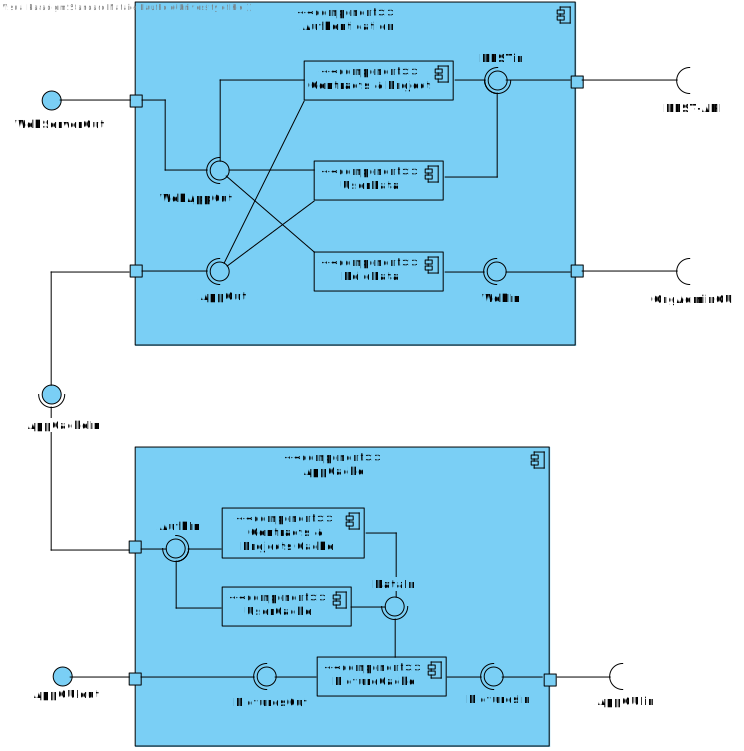
\includegraphics[width=\linewidth]{img/diagrams/cp_backend.pdf}		
	\caption{Komponentendiagramm - Backend}
	\label{fig:komponentendiagramm-backend}
\end{figure}

\begin{longtable}{|p{2.5cm}|p{10.0cm}|}
\caption{Tabelle - Komponentendiagramm-Backend}
\label{tab:table_comp_backend} \\
\hline
\textbf{Komponente} & \textbf{Beschreibung} \\ 
\hline
Authentication & Komponente, welche den eigentlichen Vorgang der Authentifizierung verwaltet. \\
\hline
AuthIn & Interface, um die Response der Authentifizierung intern in die verschiedenen Caches aufzuteilen. \\
\hline
AppCache & Komponente, welche sich um den Cache der Mobile Application kümmert, u.A. auch die Berechtigungen prüft. \\
\hline
AppGUIin & Following \\
\hline
AppGUIout & Following \\
\hline
Contracts {\&} Projects & Following \\
\hline
Contracts {\&} Projects Cache & Following \\
\hline
DataIn & Following \\
\hline
PictureCache & Following \\
\hline
PicturesIn & Following \\
\hline
PicturesOut & Following \\
\hline
REST-API & Following \\
\hline
RESTin & Following \\
\hline
RoleData & Following \\
\hline
UserData & Following \\
\hline
UserCache & Following \\
\hline
WebAppOut & Following \\
\hline
WebIn & Following \\
\hline
WebServerIn & Following \\
\hline
WebServerOut & Following \\
\hline
\end{longtable}